\begin{figure}[H]
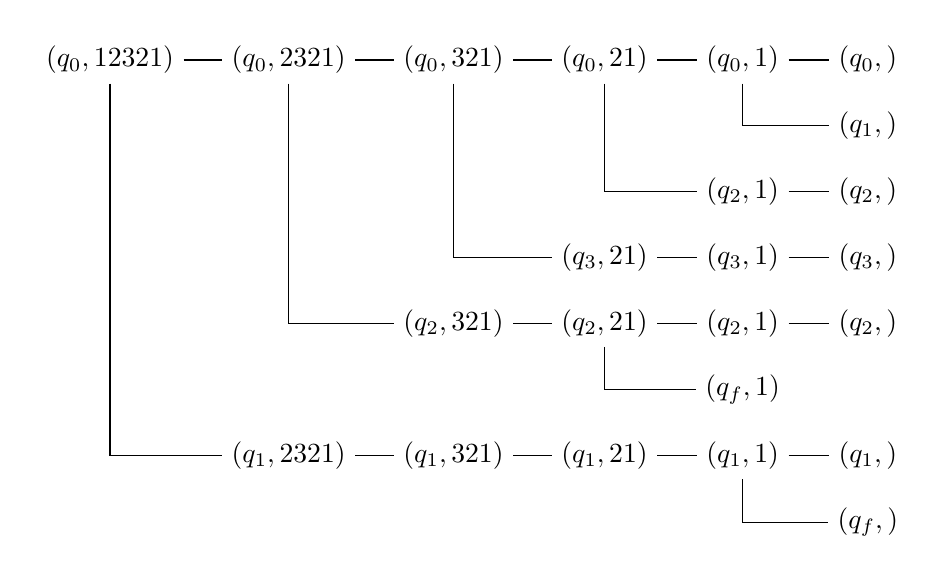
\begin{tikzpicture}
    \matrix (m1) [row sep=2.5mm, column sep=5mm]
    {
        \node (q012321) {$(q_0, 12321)$}; &
        \node (q02321)  {$(q_0, 2321)$};  &
        \node (q0321)   {$(q_0, 321)$};   &
        \node (q021)    {$(q_0, 21)$};    &
        \node (q01)     {$(q_0, 1)$};     &
        \node (q0eps)   {$(q_0, \eps)$};
        \\
        & & & & &
        \node (q1eps)   {$(q_1, \eps)$};
        \\
        & & & &
        \node (q21)     {$(q_2, 1)$};     &
        \node (q2eps)   {$(q_2, \eps)$};
        \\
        & & &
        \node (q321)    {$(q_3, 21)$};    &
        \node (q31)     {$(q_3, 1)$};     &
        \node (q3eps)   {$(q_3, \eps)$};
        \\
        & &
        \node (q2321)   {$(q_2, 321)$};   &
        \node (q221)    {$(q_2, 21)$};    &
        \node (q21X)    {$(q_2, 1)$};     &
        \node (q2epsX)  {$(q_2, \eps)$};
        \\
        & & & &
        \node (qf1)     {$(q_f, 1)$};     &
        \\
        &
        \node (q12321)  {$(q_1, 2321)$};  &
        \node (q1321)   {$(q_1, 321)$};   &
        \node (q121)    {$(q_1, 21)$};    &
        \node (q11)     {$(q_1, 1)$};     &
        \node (q1epsX)  {$(q_1, \eps)$};
        \\
        & & & & &
        \node (qfeps)     {$(q_f, \eps)$};
        \\
    };

    \draw (q012321)      -- (q02321) -- (q02321)
                          -- (q0321) -- (q021) -- (q01)  -- (q0eps);
    \draw (q01.south)    |- (q1eps);
    \draw (q021.south)   |- (q21)    -- (q2eps);
    \draw (q0321.south)  |- (q321)   -- (q31)  -- (q3eps);
    \draw (q02321.south) |- (q2321)  -- (q221) -- (q21X) -- (q2epsX);
    \draw (q221.south)   |- (qf1);
    \draw (q012321)      |- (q12321)
                          -- (q1321)  -- (q121) -- (q11)  -- (q1epsX);
    \draw (q11.south)    |- (qfeps);
\end{tikzpicture}
\caption{Схема работы автомата из примера~\ref{aut-312} на слове
$\omega=12321$.}
\label{aut-312-sch}
\end{figure}